\subsection{Approach to Benchmarking}
\label{sec:benchmarks}

Our approach to benchmarking has been incremental: starting from a very simple model and then gradually increasing the complexity. The benchmarks run so far are part of the assessment of the current parallel implementation. They also serve as a useful way of ensuring that FLAME and its generated applications are portable over a wide range of hardware and operating systems. 

\begin{table}[ht]
 \centering
  \begin{tabular}{l|ccc}
  Model     & Agents & Messages & Population   \\\hline
   Circles     &   1    &   1      &  10$^5$    \\
   C@S       &   3    &   9      &  124,000 \\
   Labour Market &   4    &   10     &  110,101 \\ 
   Bielefeld     &   4    &   29     &  43100     \\\hline
   \end{tabular}
   \caption{Details of Current Benchmark Models}
 \end{table}

The starting populations have been generated using the initial population generator developed by STFC. The ratio of agent numbers in each population was retained from the original values.

Each benchmark has been run on a variety of HPC systems available to STFC using a range of process numbers: 4 9 16 32 49 64 81 and 100. The results presented show how the elapsed time per iteration varies with number of processors. In these experiments a round-robin initial distribution has been used for the Labour Market and Bielefeld models, while geometric partitioning has been used for the Circles and C@S models.

\subsection{The Circles Model}

The Circles agent is very simple. It has a position in two-dimensional space and a radius of influence. Each agent will react to its neighbours within its interaction radius repulsively. So given a sufficient simulation time the initial distribution of agents will tend to a field of uniformly spaced agents.

Each agent has $x$, $y$, $fx$, $fy$ and $radius$ in its memory and has three states: outputdata, inputdata and move. The agents communicate via a single message board, $location$, which holds the agent $id$ and position.

The Circles problem is very simple but allows us an initial assessment of the performance of the parallelisation within FLAME. The simulation was started with a populations of $10^5$  agents and experiments performed using from 4 to 100 processors. The averaged results are shown in Table~\ref{tab:ExecutionTimesForCircles} and Figure~\ref{fig:Circles-graph}.
%Some place markers

{
\renewcommand{\arraystretch}{1.25}
\begin{table}[ht]
 \centering
  \begin{tabular}{c|cccc}
 Processors &SCARF  &HAPU  &HPCx  &bglogin2 \\ \hline
4 &- &1581.15 &4464.95 &7339.35 \\
9 &- &992.35 &2813.93 &4530.96  \\
16 &443.07 &524.47 &1600.15 &2507.14    \\
25 &281.30 &353.53 &1019.06 &1595.62    \\
36 &205.61 &242.17 &739.12 &1082.74     \\
49 &154.03 &173.25 &523.46 &786.60      \\
64 &116.13 &134.08 &390.13 &605.77      \\
81 &88.83 &105.35 &325.52 &484.19       \\
100 &75.20 &87.49 &256.59 &386.71       \\
 \end{tabular}
 \caption{Execution Times for $10^5$ Circles}
 \label{tab:ExecutionTimesForCircles}
\end{table}
}

\begin{figure}[ht]
 \centering
  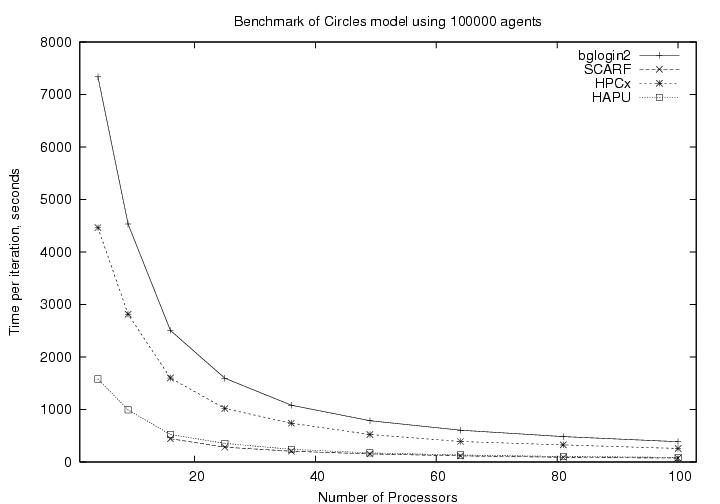
\includegraphics[width=300pt]{Circles-graph.jpg}
 \caption{Graph of iteration times}
 \label{fig:Circles-graph}
\end{figure}

The results indicate that this simulation benefits from using 30 to 50 processors after which the performance benefits flatten. It is interesting to note that this is essentially similar across the range of systems used. The variations between systems being attributed to memory, architecture and communications hardware differences.

\subsection{The C@S Model}
The C@S model was the first economic model to be implemented in FLAME by the EURACE Project.  It is based on work detailed in Delli Gatti \textsl{et al.} \cite{Delli Gatti} where an economy is populated by a finite number of \textsl{firms}, \textsl{workers}/\textsl{consumers} and \textsl{banks}. The acronym C@S stands for \textsl{Complex Adaptive Trivial System}.

This provides an initial economic model for testing FLAME. The EURACE version of C@S contains models for consumption goods, labour services and credit services. The population is a mix of agents: \textsl{Malls}, \textsl{Firms} and \textsl{People}. Each of these has different states and communicates with other agents in the population through 9 message types.

As the agents in the C@S Model have some positional/location data and the communication is localised, the initial distribution of agents to processors, as in the Circles Model, can be based on location. This helps reduce cross-processor communication.

The initial population contained: 20000 firms, 100000 people and 4000 malls (124000 agents in total).

{
\renewcommand{\arraystretch}{1.25}
\begin{table}[ht]
 \centering
  \begin{tabular}{c|cccc}
 Processors &SCARF &HAPU &HPCx  &bglogin2 \\ \hline
4 &2223.86 &3062.12 &- &-       \\
9 &1462.14 &2014.56 &- &-       \\
16 &913.52 &1159.32 &- &4888.57 \\
25 &592.44 &755.84 &2235.92 &3138.71    \\
36 &416.84 &534.62 &1589.53 &2165.96    \\
49 &307.15 &411.32 &1178.06 &1600.83    \\
64 &260.53 &313.39 &910.23 &1218.58     \\
81 &207.25 &261.33 &723.87 &992.43      \\
100 &169.46 &207.52 &601.24 &806.16     \\
 \end{tabular}
 \caption{Execution Times for C@S Model}
 \label{tab:ExecutionTimesForC@S}
\end{table}
}

%\bigskip
\begin{figure}[ht]
 \centering
  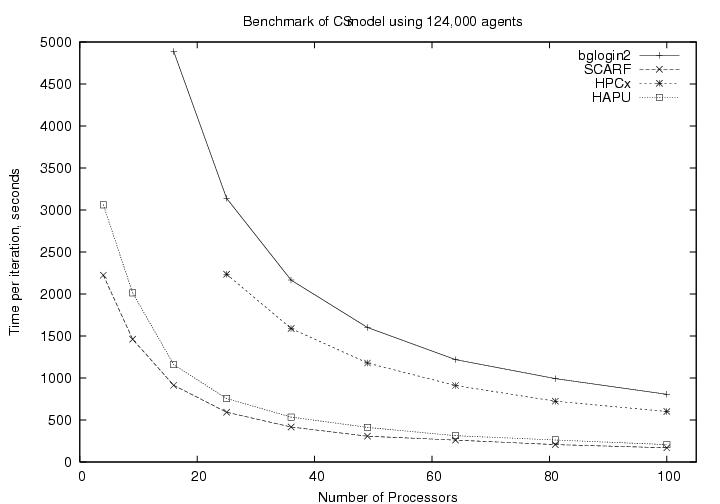
\includegraphics[width=300pt]{C@S2-graph.jpg}
 \caption{Graph of C@S Model execution times}
 \label{fig:C@S-graph}
\end{figure}

The results show a potential reduction of the elapsed time of the simulation when using up to 30 processors.



\subsection{Initial Labour Market}

This model was first model based on the work of the EURACE project. The model represented a very simplified labour market. It contains four agent types: \textit{Firm}, \textit{Household}, \textit{Market Research} and \textit{Eurostat} and 10 message types.

{
\renewcommand{\arraystretch}{1.25}
\begin{table}[ht]
 \centering
  \begin{tabular}{c|cccc}
 Processors &SCARF &HAPU  &HPCx   &bglogin2 \\ \hline
4 &1149.21 &1388.55 &- &7014.64 \\
9 &585.19 &627.45 &2317.21 &3120.96     \\
16 &334.17 &352.51 &1332.30 &1755.93    \\
25 &198.85 &233.35 &841.33 &1129.25     \\
36 &291.00 &160.97 &612.14 &782.70      \\
49 &206.82 &119.66 &449.91 &574.50      \\
64 &90.67 &97.81 &352.29 &440.36        \\
81 &72.51 &74.81 &273.78 &349.31        \\
100 &60.79 &61.34 &218.11 &284.29       \\
 \end{tabular}
 \caption{Execution Times for Labour Market Model}
 \label{tab:ExecutionTimesForLabour}
\end{table}
}
%\bigskip

\begin{figure}[ht]
 \centering
  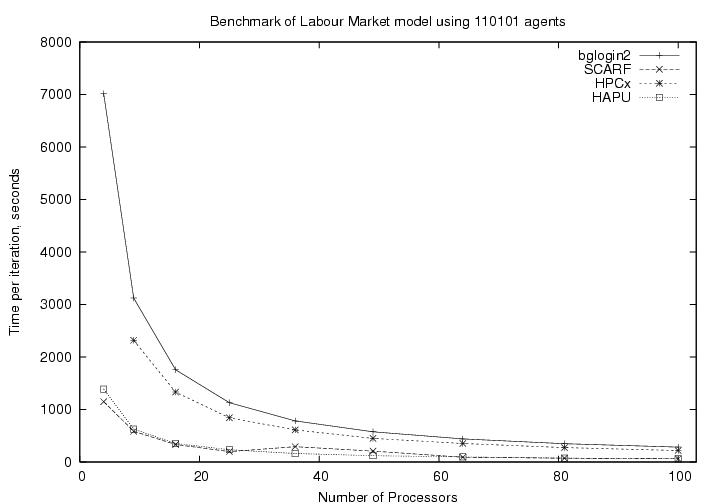
\includegraphics[width=300pt]{Labour2-graph.jpg}
 \caption{Graph of Labour Market Model iteration times}
 \label{fig:Labour-graph1}
\end{figure}

\subsection{Bielefeld Labour Market}

This model is a refinement of the Initial Labour Market. It too contains four agent types, \textit{Firm}, \textit{Household}, \textit{Mall} and \textit{Investment Goods Producer} and has 27 message types.

{
\renewcommand{\arraystretch}{1.25}
\begin{table}[ht]
 \centering
  \begin{tabular}{c|cccc}
 Processors &SCARF &HAPU &HPCx   &bglogin2 \\ \hline
4 &1078.51 &1344.86 &3253.83 &- \\
9 &542.11 &616.52 &1485.97 &-   \\
16 &318.55 &362.18 &847.84 &1173.15     \\
25 &256.06 &231.78 &552.62 &753.00      \\
36 &178.75 &162.90 &386.80 &525.79      \\
49 &119.29 &124.79 &288.37 &390.83      \\
64 &93.39 &99.91 &222.95 &299.56        \\
81 &71.06 &75.00 &179.58 &239.38        \\
100 &65.59 &61.18 &144.97 &194.95       \\
 \end{tabular}
 \caption{Execution Times for Bielefeld Model}
 \label{tab:ExecutionTimesForBielefeld}
\end{table}
}
%\bigskip

\begin{figure}[ht]
 \centering
  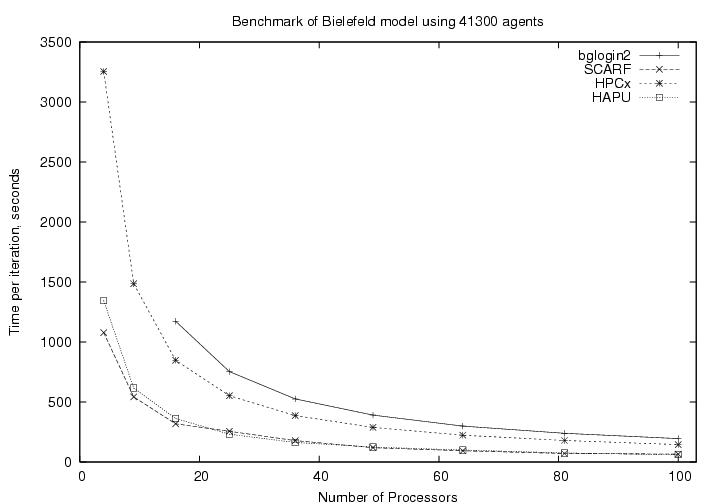
\includegraphics[width=300pt]{Bielefeld2-graph.jpg}
 \caption{Graph of Bielefeld Model iteration times}
 \label{fig:Labour-graph2}
\end{figure}

\subsection{EURACE Models}

During the development of the EURACE Model a number of domain specific models have been developed. These models were then integrated into the EURACE Model. Three domain specific models were developed: Credit Market, Labour Market and Financial Market. Each of these and the combined EURACE Model are the major economic models developed by EURACE. As part of the development of FLAME these models have been used to test the FLAME application generation and the framework infrastructure. In particular they have been very useful in testing the parallel implementation of FLAME. Although the initial agent populations is these models are very small they do encapsulate the full range and complexity of the EURACE model and to that end they are a very useful testing resource.

\begin{table}[ht]
 \centering
  \begin{tabular}{l|ccc}
  Model & Agents & Messages & Population \\\hline
  Financial Market  &    4    &   6       &  1104          \\
  Labour Market   &   7     &    45      &   1236         \\
  Credit Market   &   3     &    12      &   110         \\ 
  EURACE Model    &   9     &    54       &  2029         \\\hline
  \end{tabular}
  \caption{Details of Current EURACE Models}
\end{table}

All these models have been successfully parsed, compile and executed in both serial and parallel on some of our target HPC machines.

\clearpage

